\documentclass{article}
\usepackage{pgf}
\usepackage{tikz}
\usepackage[a3paper, landscape, margin=2in]{geometry}
\usetikzlibrary{arrows,automata}
\usepackage[latin1]{inputenc}
\pagenumbering{gobble}
\begin{document}
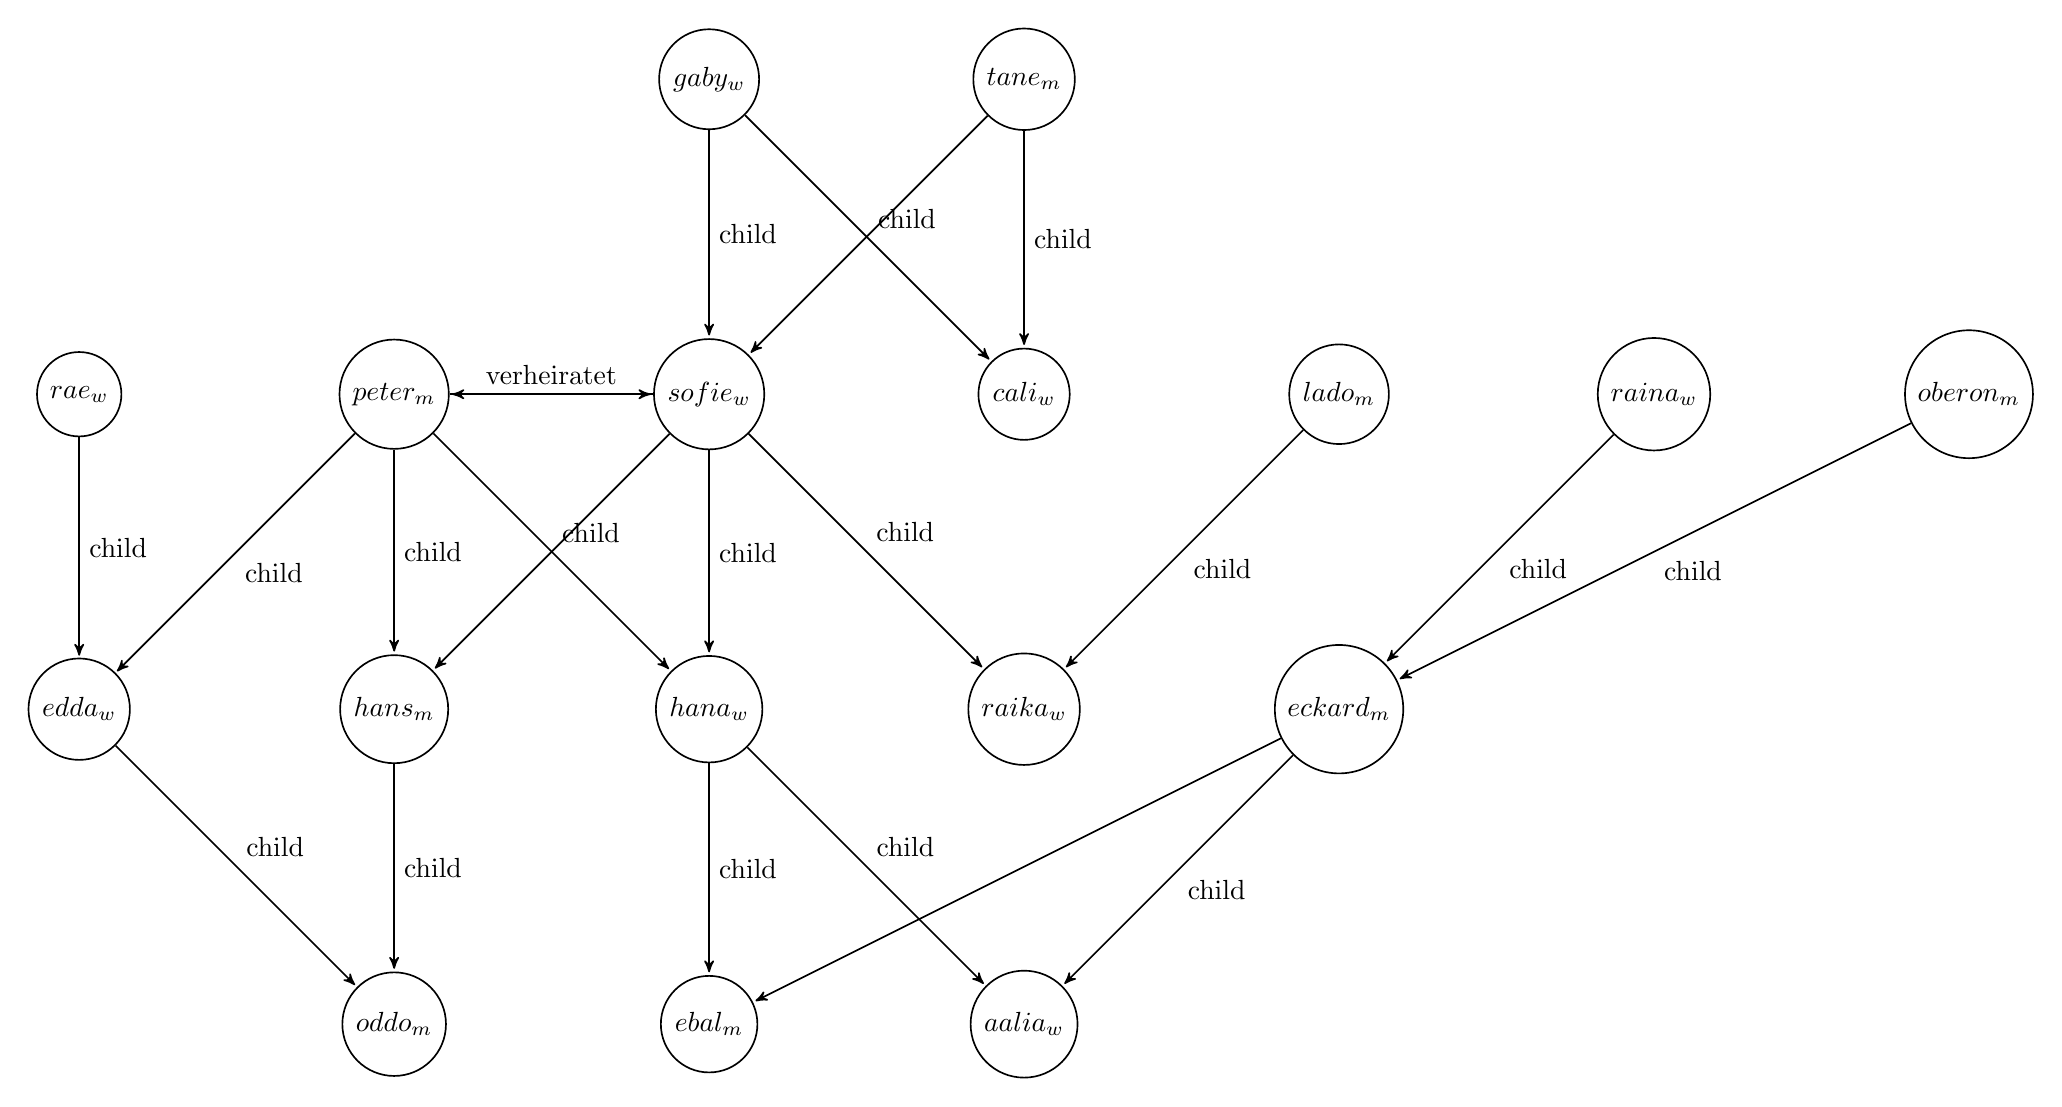
\begin{tikzpicture}[->,>=stealth',shorten >=1pt,auto,node distance=4cm,
                    semithick]
  \tikzstyle{every state}=[fill=white,draw=black,text=black]

  \node[state]			(A)                    	{$peter_m$};
  \node[state]          (B) [right of=A] 		{$sofie_w$};
  \node[state]          (C) [below of=A]		{$hans_m$};
  \node[state]          (E) [left  of=C]  		{$karl_m$};
  \node[state]          (H) [right of=C]       	{$hana_w$};
  \node[state]          (I) [above of=E]       	{$rae_w$};
  \node[state]          (T) [right of=B]       	{$cali_w$};
  \node[state]          (J) [below of=T]       	{$raika_w$};
  \node[state]          (F) [right of=J]  		{$eckard_m$};
  \node[state]     		(D) [right of=T] 		{$lado_m$};
  \node[state]          (G) [below of=H]       	{$ebal_m$};
  \node[state]          (K) [right of=G]       	{$aalia_w$};
  \node[state]          (M) [right of=D]       	{$raina_w$};
  \node[state]          (N) [right of=M]       	{$oberon_m$};
  \node[state]          (O) [left  of=G]       	{$oddo_m$};
  \node[state]          (P) [left  of=C]       	{$edda_w$};
  \node[state]          (R) [above of=B]       	{$gaby_w$};
  \node[state]          (S) [right of=R]       	{$tane_m$};
  
  \path (A) edge              node {verheiratet} (B)
            edge              node {child} 	(C)
			edge              node {child} 	(H)
			edge              node {child} 	(E)
		(B) edge              node {} 		(C)
			edge              node {} 		(A)
			edge              node {child} 	(H)
			edge              node {child} 	(J)
		(D) edge              node {child} 	(J)
		(H) edge              node {child} 	(G)
			edge              node {child} 	(K)
		(I) edge              node {child} 	(E)
		(F) edge              node {} 		(G)
			edge              node {child} 	(K)
		(M) edge              node {child}	(F)
		(N) edge              node {child}	(F)
		(C) edge              node {child}	(O)
		(P) edge              node {child}	(O)
		(R) edge              node {child}	(B)
		    edge              node {child}	(T)
		(S) edge              node {}		(B)
			edge              node {child}	(T)
			;
\end{tikzpicture}

\end{document}